\documentclass{beamer}
\usepackage{ctex, hyperref}
\usepackage[T1]{fontenc}
\usepackage{tikz}
\usetikzlibrary{positioning, shapes.geometric}
\usepackage{tikz}
\graphicspath{{img/}}
\usetikzlibrary{calc,positioning}
% other packages
\usepackage{latexsym,amsmath,xcolor,multicol,booktabs,calligra}
\usepackage{graphicx,pstricks,listings,stackengine}
\usefonttheme[onlymath]{serif}
\usepackage{subfig}
\usepackage{subfloat}
\author{顾格非}
\title{Julia集的分析和探索}
\institute{浙江大学数学科学学院}
\date{\today}
\usepackage{Tsinghua}

% defs
\def\cmd#1{\texttt{\color{red}\footnotesize $\backslash$#1}}
\def\env#1{\texttt{\color{blue}\footnotesize #1}}
\definecolor{deepblue}{rgb}{0,0,0.5}
\definecolor{deepred}{rgb}{0.6,0,0}
\definecolor{deepgreen}{rgb}{0,0.5,0}
\definecolor{halfgray}{gray}{0.55}

\lstset{
    basicstyle=\ttfamily\small,
    keywordstyle=\bfseries\color{deepblue},
    emphstyle=\ttfamily\color{deepred},    % Custom highlighting style
    stringstyle=\color{deepgreen},
    numbers=left,
    numberstyle=\small\color{halfgray},
    rulesepcolor=\color{red!20!green!20!blue!20},
    frame=shadowbox,
}


\begin{document}

\kaishu
\begin{frame}
    \titlepage
    \begin{figure}[htpb]
        \begin{center}
            
\includegraphics[width=0.3\linewidth]{logo.jpeg}
        \end{center}
    \end{figure}
\end{frame}

\begin{frame}
    \tableofcontents[sectionstyle=show,subsectionstyle=show/shaded/hide,subsubsectionstyle=show/shaded/hide]
\end{frame}


\section{背景介绍}
\begin{frame}{Julia集合的定义}
    \begin{itemize}
        \item Julia set是一个在复平面上形成分形的点的集合。以法国数学家加斯顿·朱利亚(Gaston Julia)的名字命名。
        \item Julia集合可由$f_c(z)=z^2+c$反复迭代得到,对于固定的复数c,取某一$z$值(如$z=z_0$),可以得到序列:
$$
z_0,f_c(z),f_c(f_c(z)),f_c(f_c(f_c(z))),……
$$

这一序列可能发散于无穷大或始终处于某一范围之内并收敛于某一值。我们将使其不扩散的z值的集合称为Julia集合。
    \end{itemize}
    
\end{frame}


\section{数学理论}
\begin{frame}{数学理论}
    Julia集具有对称性,不变性和自相似性
    \begin{itemize}
        \item 如果 c 是实数,则 Julia 集围绕实轴镜像。具有非零虚部的其他 c 值具有 180 度旋转对称性。
        \item Julia 集的点对于 $f(z)$ 的进一步迭代是“不变的”。这里,不变性并不意味着 $f(z_j )=z_j$,而是对于属于集合$J$的任何点$z_j$ ,$f(z_j)$ 也是$J$的成员。
        \item 在图片的每个微小的局部,都和整个图形的样子相似。
    \end{itemize}
\end{frame}


\section{计算机实现}


\begin{frame}{算法介绍}
    算法设计思路:
    \begin{itemize}
        \item 设定一个迭代次数的上限$N$ ,当经过 $N$次迭代,$f_c(z)$仍然没有超过 2,我们就认为这个点就属于Julia集合 (尽管一些点也可能混入Julia集合);否则,就说明该点不Julia集合在中,并记录这个点挑出循环时的次数。
        \item 这样平面上每个点都对应了一个循环次数$i$(对于集合内的点,$i=N$;对于集合外的点,$i<N$),然后将$i$映射到颜色上去进行着色。
    \end{itemize}
\end{frame}


\begin{frame}{流程图}
   \begin{center}
\begin{tikzpicture}[node distance=8pt]
  \node[draw, rounded corners]                        (start)   {输入某个复数c};
  \node[draw, below=of start,align=center]                         (step 1)  {遍历所有的复数$z_0$ \\ 循环计数器i=1};
  \node[draw, below=of step 1,align=center]                        (step 2)  {$z=z^2+c$\\i=i+1};
  \node[draw, diamond, aspect=2, below=of step 2,align=center]     (choice)  {$z<2?$\\$i\leq N?$ };
  
  \node[draw, rounded corners, below=of choice]  (end)    {记录挑出循环的i};
  \node[draw, rounded corners, below=of end]  (end2)     {根据i的大小映射到不同的颜色};
  
  \draw[->] (start)  -- (step 1);
  \draw[->] (step 1) -- (step 2);
  \draw[->] (step 2) -- (choice);
  \draw[->] (choice) -- node[left]  {No} (end);
  \draw[->] (choice.east)--($(choice.east)+(1,0)$) --node[left]{Yes}  ($(step 2.east)+(1.8,0)$) -- (step 2.east);
  \draw[->] (end) -- (end2);
\end{tikzpicture}
\end{center}
\end{frame}

\section{数值算例}
\begin{frame}{迭代过程展示}
    以下展现了一个迭代的过程。通过控制最大迭代次数$N$的增大,图形精度越来越高,红色的面积越来越小。

\begin{figure}[H]
	\centering
	\subfloat[N=5]{
	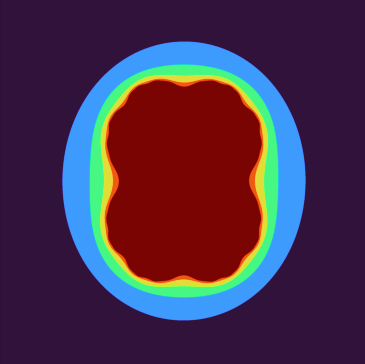
\includegraphics[width=2cm]{5.png}
	}
	\subfloat[N=15]{
	
\includegraphics[width=2cm]{15.png}
	}
	\subfloat[N=100]{
	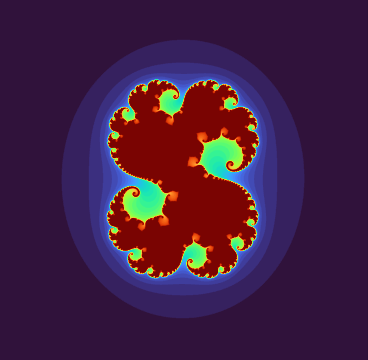
\includegraphics[width=2cm]{0.273_0.007.png}
	}
	\caption{不同迭代次数下$c=0.273+0.007i$的图像}
\end{figure}
\end{frame}


\section{与mandelbrot的关系}
\begin{frame}{与mandelbrot的关系}
    \begin{itemize}
        \item 众所周知的 Mandelbrot 集形成了 Julia 集的一种索引。一个 Julia 集要么是连通的,要么是不连通的。\item 从 Mandelbrot 集合内选择的 c 值是连通的,而从 Mandelbrot 集合外部选择的 c 值是不连通的。
        \item 不连贯的集合通常被称为“dust”,无论以何种分辨率查看它们,它们都由单个点组成。
    \end{itemize}
    
\end{frame}
\begin{frame}
    \begin{center}
        {\Huge\calligra Thanks!}
    \end{center}
\end{frame}

\end{document}
